\documentclass[a4paper, 11pt, hidelinks]{article}
\usepackage{bookmark}
\usepackage[utf8]{inputenc} 
\usepackage[T1]{fontenc}
\usepackage{lmodern}
\usepackage{graphicx}
\usepackage[french]{babel}
\usepackage{geometry}
\usepackage{eucal}
\usepackage{caption}
\usepackage{float}
\usepackage{url}
\usepackage{amsmath}
\usepackage{amssymb}
\usepackage{color}
\usepackage{hyperref}
\usepackage{cancel}
\usepackage{tikz}
\usepackage{mathrsfs}  
\usepackage{esvect}
\usepackage[standard]{ntheorem}
\usepackage{romanbar}
\usepackage{titlesec}
\usepackage[final]{pdfpages}
\usepackage{xcolor}
\usepackage{xcolor, soul}


\geometry{hmargin=2cm,vmargin=1.5cm}

\tikzset{
  treenode/.style = {shape=rectangle, rounded corners,
                     draw, align=center,
                     top color=white, bottom color=blue!5},
  root/.style     = {treenode, font=\Large, bottom color=red!10},
  env/.style      = {treenode, font=\ttfamily\normalsize},
  dummy/.style    = {circle,draw}
}

\newcommand{\prp}{\large \textbf{Proposition:} \large}

\newcommand{\tm}{\large \textbf{Théoreme:} \large}

\newcommand{\ex}{\textcolor{green}{Exemple:} }

\newcommand{\dm}{\textcolor{red}{\textbf{Démo:} } }

\newcommand{\de}{\large \textbf{Définition} \large }

\newcommand{\rmq}{\textbf{Remarque:} }

\newcommand{\bs}{\bigskip}

\newcommand{\voca}{\textcolor{blue}{\textbf{Vocabulaire} } }

\newcommand{\lem}{\textcolor{red}{\textbf{Lemme:} } }

\newcommand{\rb}[1]{\Romanbar{#1}}

\newcommand{\cit}{\textcolor{blue}{\textbf{Citation: }}}

\definecolor{authorGray}{RGB}{20,20,20}
\definecolor{citationRed}{RGB}{255,110,110}
\definecolor{surlignage}{RGB}{255,249,151}

\newcommand{\citer}[3]{\bs \begin{center} \textcolor{authorGray}{#1 :} \textcolor{citationRed}{\og #2 \fg} \textcolor{authorGray}{(\underline{#3})} \end{center} \bs}

\newcommand{\trinom}[3]{\begin{pmatrix}
    #1 \\
    #2 \\
    #3
\end{pmatrix}}

\newcommand{\quadrinom}[4]{\begin{pmatrix}
    #1 \\
    #2 \\
    #3 \\
    #4 \\
\end{pmatrix}}

\newcommand{\pentanom}[5]{\begin{pmatrix}
    #1 \\
    #2 \\
    #3 \\
    #4 \\
    #5
\end{pmatrix}}

\newcommand{\hexanom}[6]{\begin{pmatrix}
    #1 \\
    #2 \\
    #3 \\
    #4 \\
    #5 \\
    #6 
\end{pmatrix}}

\newcommand{\serie}[2]{\displaystyle\sum_{#1 =0}^{+\infty} #2_{#1} }

\newcommand{\tend}{\underset{n \to+ \infty}{\longrightarrow} }

\newcommand{\Lra}{\Leftrightarrow}

\newcommand{\lra}{\leftrightarrow}

\newcommand{\Ra}{\Rightarrow}

\newcommand{\ra}{\rightarrow}

\newcommand{\la}{\leftarrow}

\newcommand{\La}{\Leftarrow}

\newcommand{\dsum}[2]{\displaystyle\sum_{#1}^{#2} }

\newcommand{\dint}[2]{\displaystyle\int_{#1}^{#2} }

\newcommand{\ntend}{\underset{n \to+ \infty}{\not\longrightarrow} }

\newenvironment{lmatrix}{$ \left|\begin{array}{l} }{\end{array}\right.$}


\newcommand{\img}[4]{\begin{figure}[!ht]
    \centering
    \includegraphics[scale=#1 ]{#2}
    \caption{#3}\label{#4}
    \end{figure} }    
\begin{document}

\newcommand{\grad}[1]{\vv{grad}#1}

\sethlcolor{surlignage}

\title{Cours- Français- Philosophie- Le travail}
\author{Schobert Néo}

\maketitle

\tableofcontents


\newpage

\part{Introduction}


\section{Le travail expliqué par les mythes: une notion ambivalente}

\subsection{Epiméthée et Prométhée}

\subsubsection{Contexte général du mythe}

\begin{itemize}
    \item Epiméthée et Prométhée sont les fils d'un Titan Japet, lui-même issu de Gaïa et Ouranos.
    \item Pour récompenser Epiméthée et Prométhée après la guerre contre son père, il leur confie la tâche d'organiser le vivant.
    \item Il y a une version d'Hésiode, mais la version étudiée ici est celle de Platon.
\end{itemize}




\subsubsection{L'homme, animal à part dans la nature}

\begin{itemize}
    \item Après avoir organisé le vivant, Epiméthée se rend compte qu'il n'a donné aucun attribut à l'homme.
    \item Prométhée vole alors un attrivut divin: le feu sacré; pour le donner à l'homme, qui n'a rien.  L'homme acquiert
    donc la technique et le travail humain.
    \item  L'homme devient alors la créature la plus puissante du vivant.
    \item Avec l'intelligence pratique, la \og raison instrumentale \fg , l'homme reçoit la capacité de fabriquer de 
    manière artificielle l'ensemble des attributs distribués au vivant.
    \item Le travail devient pour l'homme le moyen de subvenir artificiellement à ses besoins et de s'extraire à la nature.
    \item L'homme devient par ce travail un producteur de culture. L'homme sublime par le travail sa nature animale.
    \item Le travail est un propre de l'homme.
    \item La faiblesse de l'homme fait alors sa force.
\end{itemize}


\citer{Karl Marx}{Ce qui distingue d'emblée le pire architecte de l'abeille la plus experte, c'est qu'il a construit la cellule dans sa tête avant de la construire dans la ruche.}{Le Capital}

\begin{itemize}
    \item Pour Aristote, la main est le premier outil propre à l'homme.
    \item Prométhée est un symbole des lumières (\rb{18}$^e$ siècle)
\end{itemize}

\subsubsection{La rançon du travail: faiblesse (de l'homme) et ambivalence (de la nature)}

\begin{itemize}
    \item L'homme \og arraché \fg à sa condition animale, va souffir d'un désir toujours réaffirmé, toujours plus fort de s'éloigner de cette nature animale.
    \item L'homme ne peut plus survivre qu'en transformant la nature / son environnement et donc en le détruisant. C'est pour cela que le vol de Prométhée 
    constitue une faute / un sacrilège. L'homme se retrouve entre deux mondes: le monde divin et le monde animal.
\end{itemize}




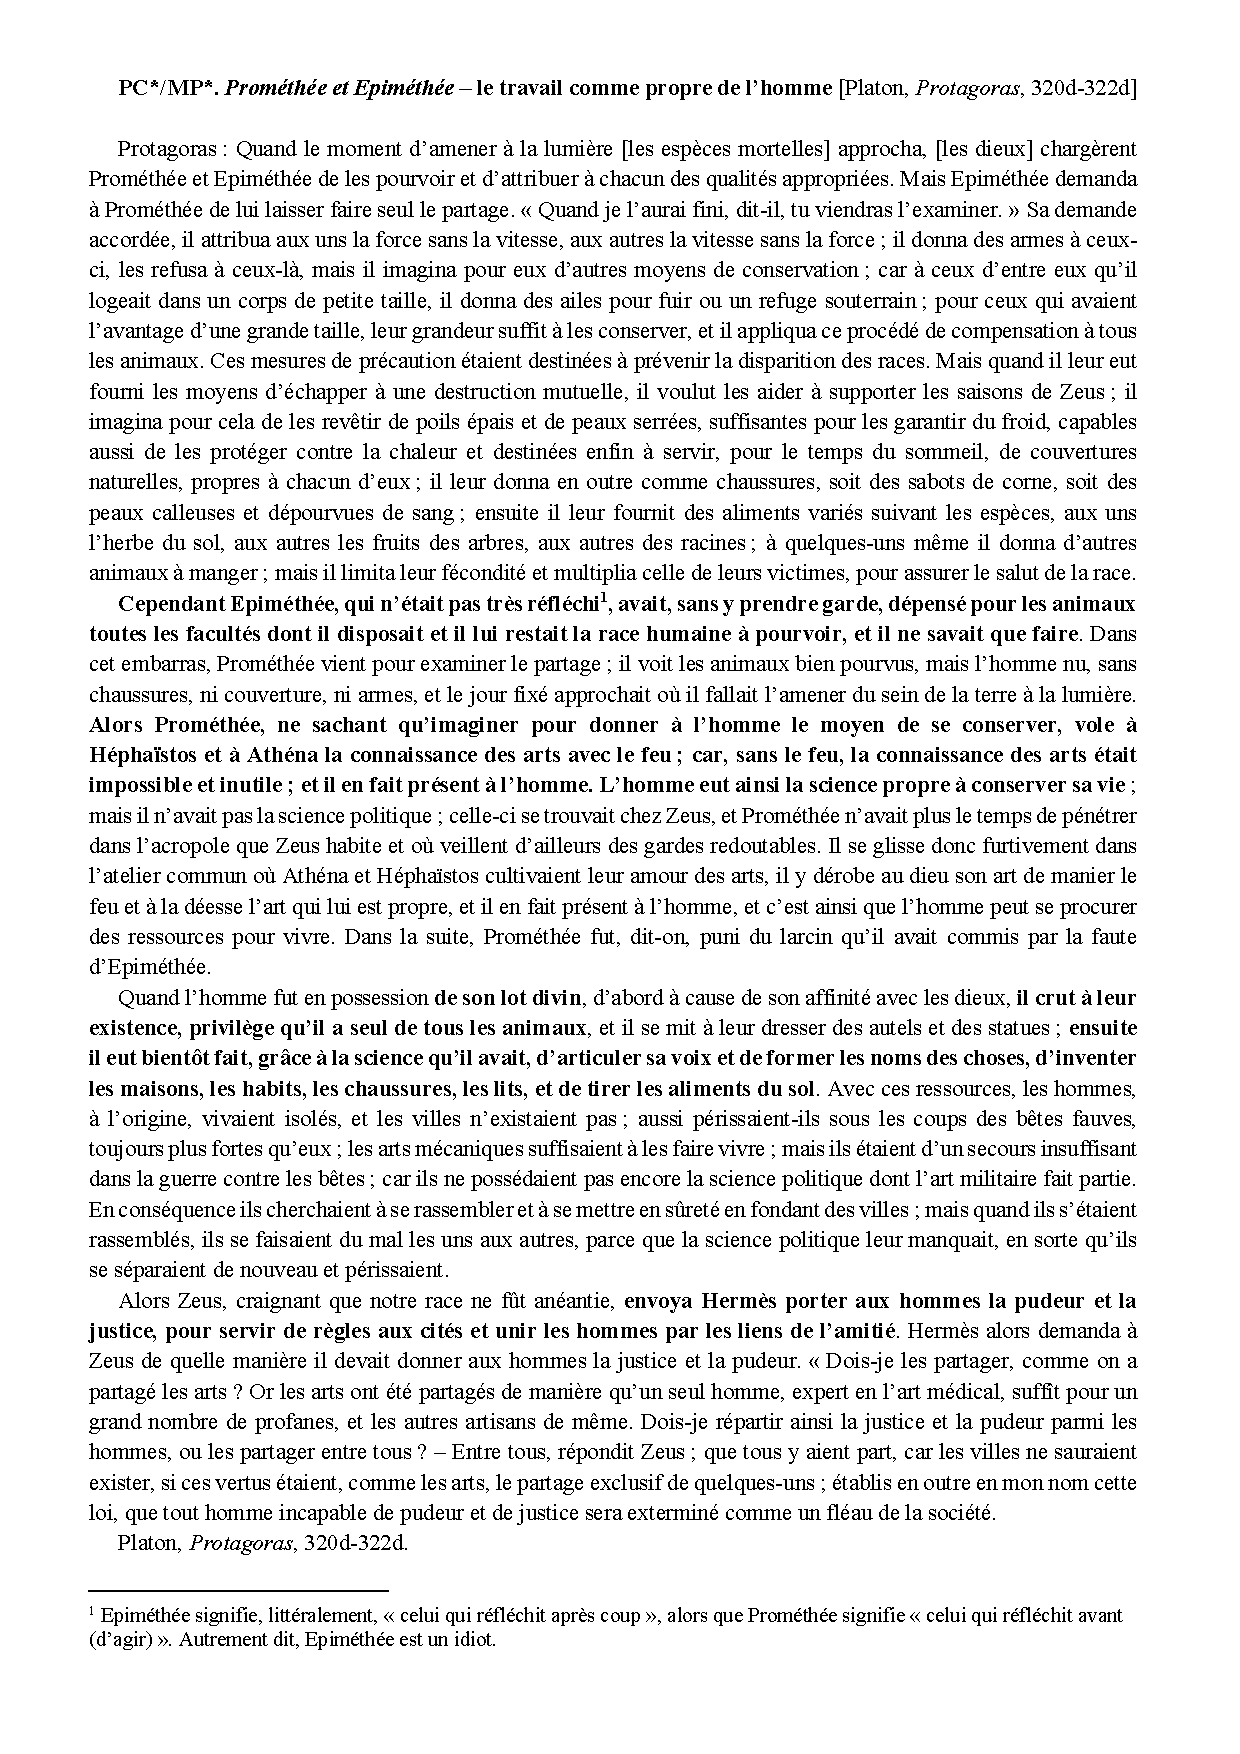
\includepdf[pages=-]{I. A. Promethee Epimethee.pdf}


\subsection{Travail, hybris, civilisation}

\begin{itemize}
    \item Le travail (et la technique) pour les Anciens n'est ni bon ni mauvais (les deux en même temps), il doit s'inscrire dans un cadre éthique [des règles communes 
    visant à préserver l'équilibre, l'harmonie].
    \item Mais alors pourquoi cet enjeux ? 
        \begin{itemize}
            \item Le travail nous rapproche des dieux et nous fait oublier notre condition animale.
            \item Cet enjeu mène à un risque d'hybris [= la \og démesure \fg en grec]
        \end{itemize}
    \item La faute pour les Anciens, c'est de se prendre pour dieu en voulant dépasser sa condition.
    \item Celui qui fait d'hybris est toujours puni, Prométhée par exemple est châtié (il est enchaîné sur un rocher du Caucase: un aigle chaque jour
    lui dévorant le foie).
\end{itemize}

\citer{Hérodote}{Le ciel rabaisse toujours ce qui dépasse la mesure}{Source inconnue}

Exemple d'hybris:
\begin{itemize}
    \item Icare, fils de Dédale (architecte) qui a rendu service à Minos (roi de Crête), dont la femme a enfanté
    un monstre mi-homme, mi-taureau (Minotaure). Dédale construit un labyrinthe pour \og cacher \fg le Minotaure. Minos abandonne
    Dédale et son fils dans le labyrinthe. Dédale construit alors des ailes ($1^{ere}$ faute) (métamorphose de la condition humaine)
    pour Icare. Icare, séduit par l'attrait du soleil et par l'ivresse de sa toute puissance, oublie sa condition d'homme et se rapproche du soleil.
    Ses ailes fondent alors, Icare chute et meurt.
\end{itemize}

\bs

\begin{itemize}
    \item On comprend que pour les Anciens, le travail s'inscrit dans un \og ordre du monde \fg plus général.
    \item Cet ordre est celui voulu / garanti par tous. 
    \item Dans la cosmogonie \og gréco-romaine \fg, il y a 3 étapes : âge de Cronos / âge de Saturne / âge de Jupiter.
    \item Jupiter établit alors la stabilité en instaurant un équilibre, ce qui est proscrit, c'est également l'hybris, qui mène aux transgressions de l'ordre.
\end{itemize}

\bs

Dans cette vision du monde, le macrocosme [ordre divin] et le microcosme [ordre humain] sont liés. Ces deux ordres sont analogues.
\begin{itemize}
    \item L'ordre humain est assuré par la mesure (rester à sa place). Dans le monde humain,
        \begin{itemize}
            \item La position \og sage \fg consiste à accepter l'humilité / la faiblesse d'une condition dévolue au travail.
            \item La position \og démesurée \fg (hybris) est celle de ceux qui, par démesure (voiloir le pouvoir, la richesse, la puissance)
            choisissent la guerre, l'affrontement, etc ... Et génère le chaos. Celui de la guerre civile dénature l'homme (frère contre frère).
            \item Le travail doit être pensé et associé à une vision de l'ordre où le quotidient résonne avec le macrocosme. Le paysan et son 
            travail n'ont pas seulement une visée \og productive \fg mais s'inscrivent dans un ordre du monde stable et harmonieux dont ils participent 
            à la réalisation.
            \item Le travail est toujours lié à un ensemble de valeurs. (humilité, amour du travail bien fait, goût de l'effort, persévérance, observation
            de la nature, etc ...)
        \end{itemize}
    \item La question de la satiété [fait dêtre repu, surabondance. \og satis est \fg : \og ça suffit \fg (je suis rempli)].
        \begin{itemize}
            \item Pour les Modernes, la satiété est positive, c'est l'incarnation d'une société matérialiste, consumériste, productiviste, qui vise
            le confort. Le bonheur est associé à l'abondance matérielle.
            \item Pour les Anciens, la satiété est soit père, soit fils de la démesure (hybris). Le travaile ne vise pas à sa propre abolition.
            \citer{Solon}{Le trop-plein engendre la démesure quand une prospérité considérable s'attache à des gens sans sagesse}{Source inconnue}
            \item La satiété est un danger :
                \begin{itemize}
                    \item Si la nécessité est complètement abolie par l'abondance, l'homme va suivre seulement son désir. Cela pose problème car le désir est irrationnel.
                    \item La satiété nous fait oublier notre condition (nos faiblesses). 
                \end{itemize}
        \end{itemize}
\end{itemize}

\subsection{Le mythe des \og races \fg / des âges chez Hésiode}


\begin{itemize}
    \item Hésiode : poète grec du \rb{18}$^e$ siècle avant notre ère (époque d'Homère)
    \item \underline{Les travaux et les jours} : Poème didactique qui porte sur la récole, l'élevage, l'observation du ciel pour établir le
    calendrier agricole, outils, animaux... C'est une source principale d'inspiration pour \underline{Les Géorgiques}.
    \item Hésiode s'adresse ici d'abord à son frère Persès, qui a tenté de lui voler sa part d'héritage (les terres).
    \item Pourquoi Persès se comporte ainsi ? Il veut pouvoir ne plus travailler.
    \item Hésiode dit à Persès. \citer{Hésiode}{que l'envie ne te détourne pas du travail.}{Source inconnue}
    \item Hésiode va tenter de le raisonner à travers un récit mythologique qui explique que l'hybris génère le chaos et 
    que le travail est la condition même de l'homme.
\end{itemize}

\bs

\bs

Résumé des âges:
\bs

\begin{itemize}
    \item $1^{er}$ Âge: Âge d'or
    \begin{itemize}
        \item Monde sans travail
        \item Temps béni
        \item Les hommes ne souffrent pas
        \item Âge vertueux (partage, respect des dieux)
    \end{itemize}
    \item $2^e$ Âge: Âge d'agent   
    \begin{itemize}
        \item Bêtise
        \item Vice 
        \item Hybris: les hommes ne respectent pas les dieux
        \item Injustice : mène à la souffrance
    \end{itemize}
    \item $3^e$ Âge: Âge d'airain
    \begin{itemize}
        \item Hommes forts, puissants
        \item Mais hommes injustes : mène à l'hybris et les hommes s'entretuent
        \item Vice 
    \end{itemize}
    \item $4^e$ Âge: Âge des héros
    \begin{itemize}
        \item Hommes forts, puissants
        \item Hommes plus vertueux, qui consacrent leur vie à la guerre, qui meurent
        \item Ce sont des héros de la mythologie.
    \end{itemize}
    \item $5^e$ Âge: Âge de fer
    \begin{itemize}
        \item Monde où les hommes souffrent
        \item Où le bien et le mal son mélangés
        \item La justice dépend alors des hommes
    \end{itemize}
\end{itemize}



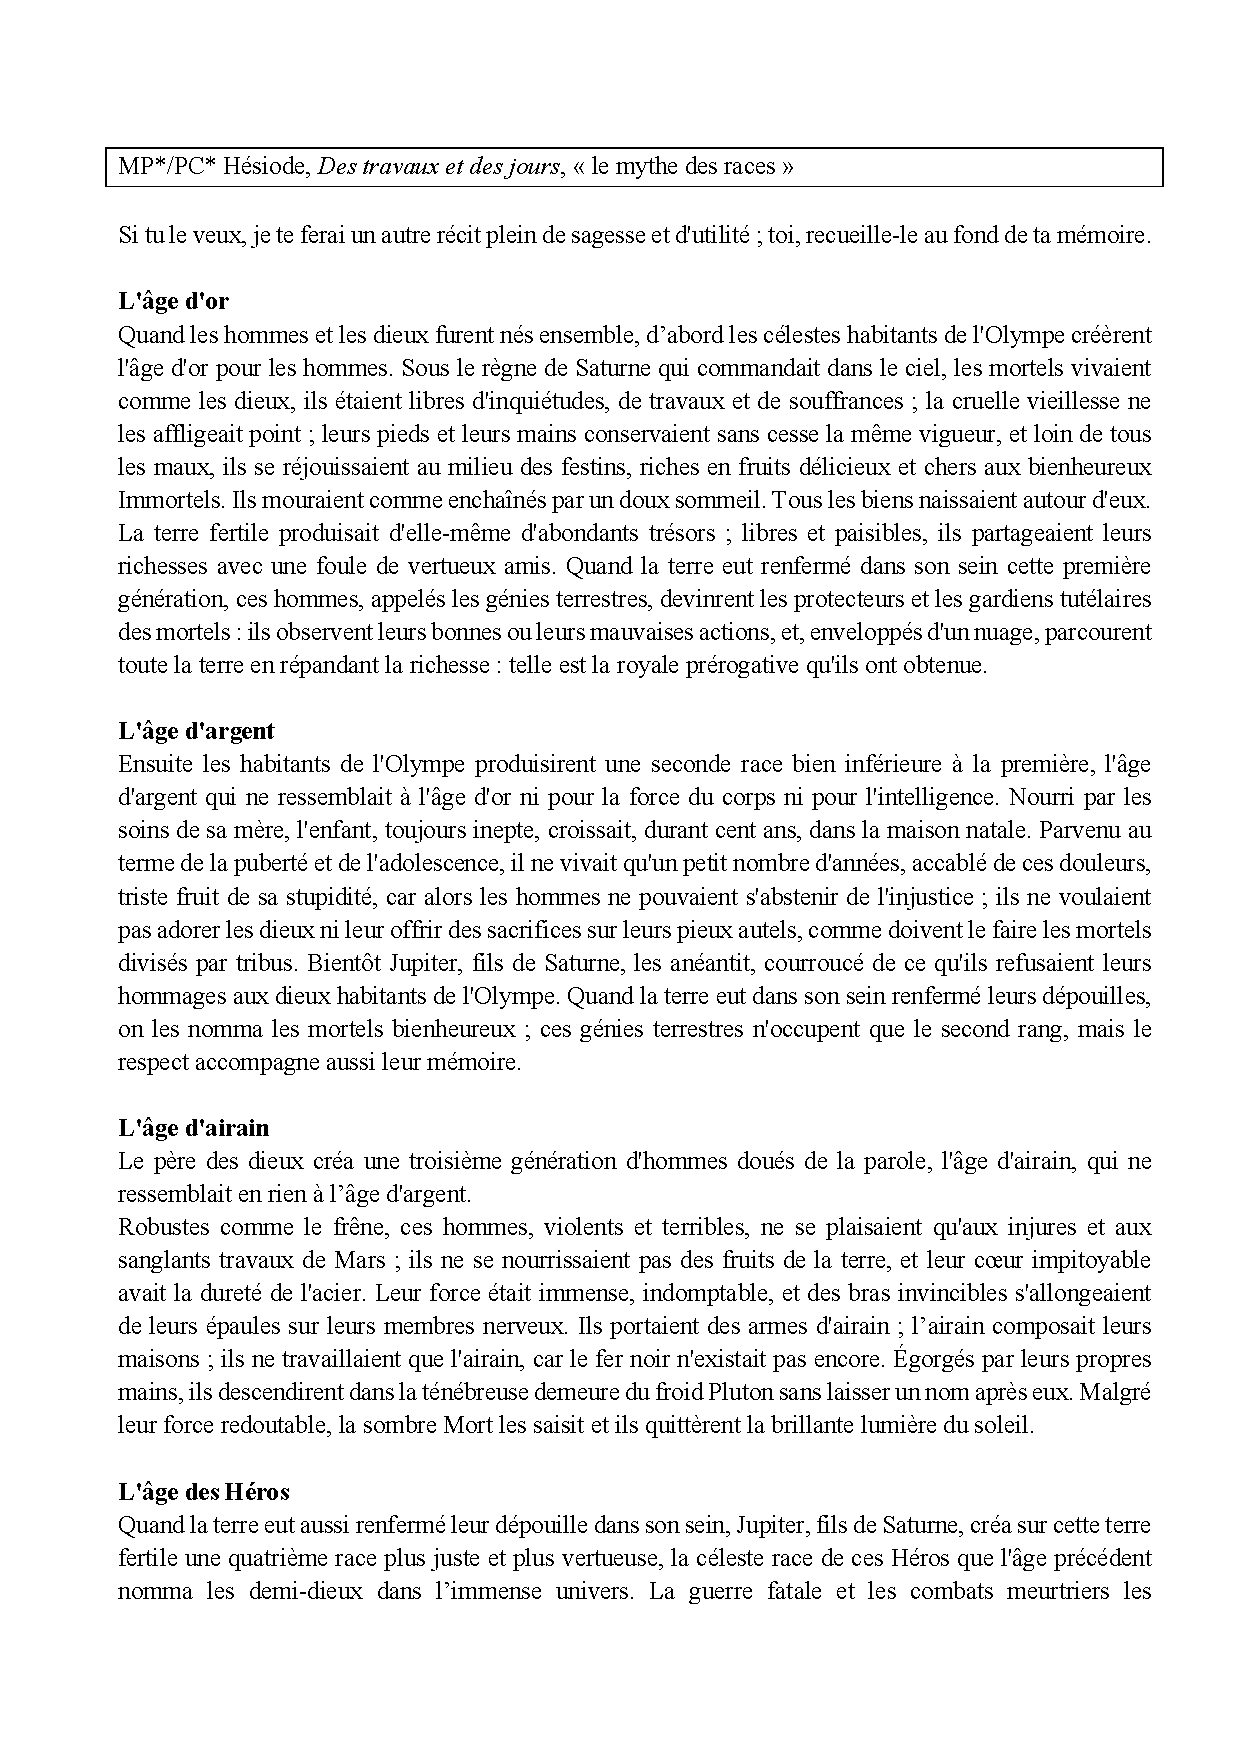
\includepdf[pages=-]{I. B. Hesiode mythe des races.pdf}


\begin{itemize}
    \item Hésiode dit à son frère que chaque fois que l'homme de fer commet l'injustice (hybris), il risque de déclencher la colère de Zeus
    et la destruction du monde, et le départ de \og Justitia \fg vers le ciel.
    \item Zeus risque de détruire ce monde quand l'hybris va l'emporter, quand le père sera contre le fils et que les frères seront contre les frères.
\end{itemize}

\bs

Récapitulatif:

\fbox{%
\begin{minipage}{0.75\textwidth}
    \begin{itemize}
        \item Âge d'or: vertueux
        \item Âge d'Argent: hybris
    \end{itemize}    
\end{minipage}
}

\fbox{%
\begin{minipage}{0.75\textwidth}
    \begin{itemize}
        \item Âge d'airain: hybris
        \item Âge des héros: vertueux
    \end{itemize}    
\end{minipage}
}

\fbox{%
\begin{minipage}{0.75\textwidth}
    \begin{itemize}
        \item Âge de fer: âge actuel, \og mêlé \fg. Règne aussi bien l'injustice que le juste.
    \end{itemize}    
\end{minipage}
}

\bs 

Si les humains choisissent la démesure, alors Justitia va s'envoler et quitter la Terre.

\bs

Hésiode utilise un argument religieux pour rappeler son propre frère à la mesure (La démesure humaine produit le chaos). D'où 
la vision binaire de l'âge de fer. 

\bs

Il s'agit d'un tableau diptyque [tableau en 2 parties]
\begin{itemize}
    \item Utopique
    \item Dystopique: 
    \begin{itemize}
        \item Hommes remplis d'hybris, marqué par la gloire, le pouvoir, la conquête, l'absence de travail, la guerre, l'appropriation
        de biens par la violence. Ces hommes pleins d'hybris produisent / provoquent le chaos, l'impiété, la stérilité.
    \end{itemize}
\end{itemize}

\bs

Cela rappelle aussi l'histoire du vieillard qui a reçu une terre \og abandonnée \fg. Virgile, \underline{Les Géorgiques}, Livre \rb{4}, p $152$.

\subsection{Mythe chrétien du travail dans la Génèse.}


La Génèse est l'autre grand récit qui alimente la réflexion de l'Occident sur le travail: il présente le travail comme une réalité
ambivalente, entré bénédiction et malédiction.


\textcolor{red}{ATTENTION} à l'anachronisme: Ne pas comparer Virgile et ce récit chrétien. Il n'y a de relation entre les deux: Virgile ne 
connait pas la Bible (même si c'est à peu près la même époque quoique Virgile était sûrement un peu avant, il n'en a pas entendu parler)


\begin{itemize}
    \item $1^e$ étape : (Création)
    \begin{itemize}
        \item Création, l'homme est placé dans un jardin paradisiaque et fertile (jardin d'Eden)
        \item Dieu lui donne une mission bénie: \og garder et cultiver \fg le jardin. L'homme est ménager
        de la nature et ne souffre pas de ce travail.
        \item Dieu fait de l'homme son \og protégé \fg : l'homme est supérieur aux autres vivants et doit les 
        soumettre. Dieu confère à l'homme une partie de son pouvoir: celui de nommer les animaux.
        \item Au début, le travail est alors béni.
    \end{itemize}
    \item $2^e$ étape : (Chute originelle)
    \begin{itemize}
        \item Récit de la désobéissance des hommes à Dieu qui va entraîner la \og chute \fg, c'est-à-dire l'expulsion du jardin d'Eden.
        Ils veulent accéder à la connaissance du bien et du mal qui est une prérogative divine: l'homme veut s'élever au-dessus de sa condition.
        \item Il est puni par la souffrance désormais associée au travail : 
        \begin{itemize}
            \item Souffrance dans le travail qui produit la vie (\og enfanter dans la douleur \fg)
            \item Souffrance dans le travail qui permet de subsister.
        \end{itemize}
    \end{itemize}
\end{itemize}



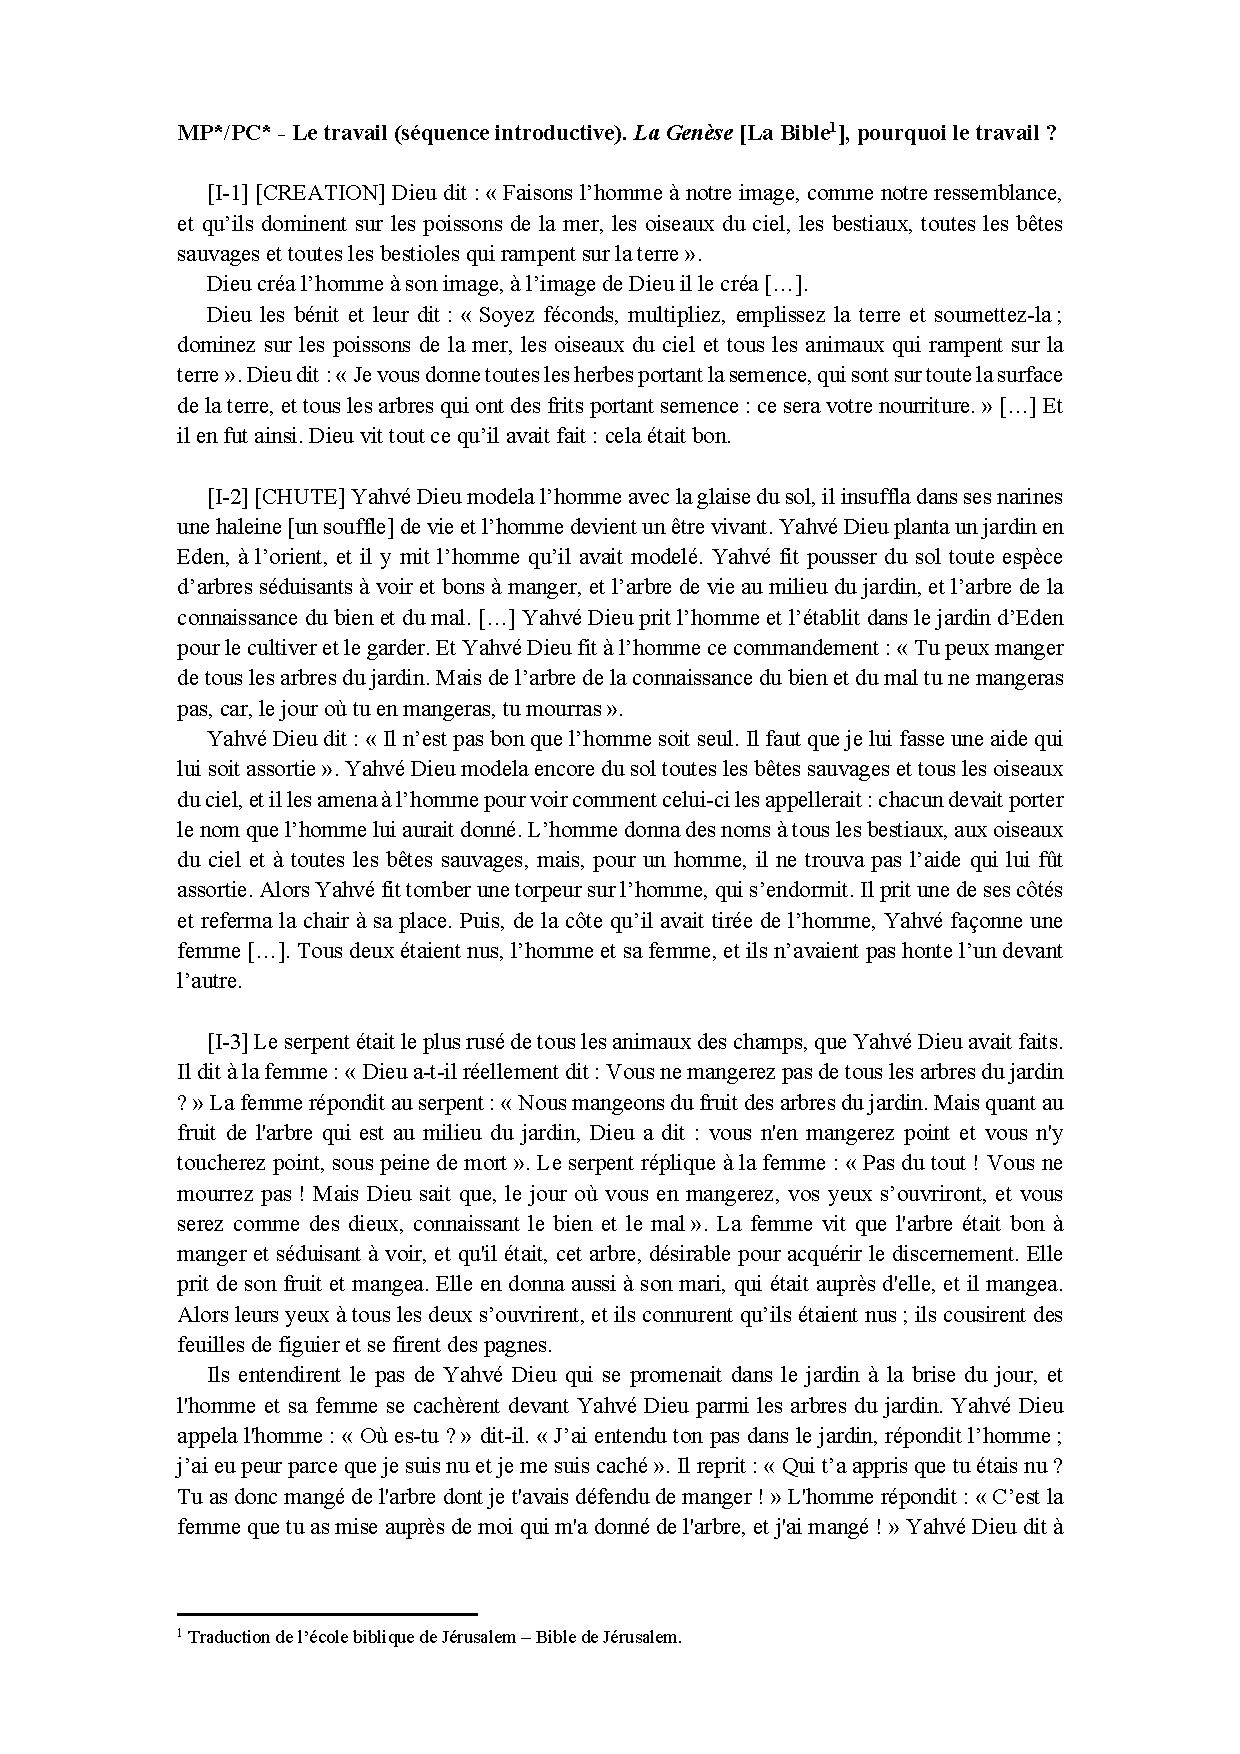
\includepdf[pages=-]{I. C. Genese Le travail.pdf}


Dans la Bible, la vie de l'homme est consacrée au travail mais il y a deux visions: 

\begin{itemize}
    \item Le travail est bien quand l'homme participe à la création, à l'\oe uvre de Dieu. Par son travail, l'homme peut essayer de
    rétablir l'harmonie qu'il a lui-même brisé et dont il porte la faute. Expiation de la faute originelle. La souffrance permet cette
    expiation (\og dolorisme \fg)
    \item Le travail est mauvais s'il répond à un souci \og individualiste \fg, dans l'oubli de Dieu. Un travail centré sur la richesse, sur
    le pouvoir, (etc ...) est perçu comme la continuation / perpétuation de la \og faute \fg originelle. 
\end{itemize}


Le terme \og travail \fg émerge à l'époque médiévale (et remplace les autres mots comme \og labeur \fg (labor)):
\begin{itemize}
    \item Ce mot induit en effet l'idée de souffrance.
    \item \og tri-palium \fg : instrument de torture composé de $3$ pieux.
\end{itemize}


En certitude judéo-chrétien : il y a une dimension sacrificielle dans le travail.


\begin{itemize}
    \item Somone Weil : C'est par choix qu'elle se rend à l'usine. (souffrance volontaire)
    \item Vinaver : Le travail dans l'entreprise inclut une dimension sacrificielle.
\end{itemize}





\section{Histoire (moderne) du travail}

\subsection{Avant l'histoire, une \og préhistoire \fg du travail: la révolution néolithique}

\subsubsection{Révolution néolithique}

A la révolution néolithique, il y a l'invention de l'agriculture ($-10 000$ ans avant notre ère: à la fin de la dernière 
période glaciaire qui rend possible la domestication des plantes).


Il y a passage d'une économie de prédation (\og chasseurs-cueilleurs \fg nomades) à une économie de la production (sociétés rurales)


Conséquences : 
\begin{itemize}
    \item Explosion démographique : 
    \begin{itemize}
        \item - $10000$ ans : $\sim 6$ millions d'individus.
        \item - $3000$ ans : $\sim 100$ millions d'individus.
    \end{itemize}
    \item Naissance des premiers états.
    \item Début des inégalités / hiérarchies sociales.
    \item Début de la division du travail.
    \item Naissance de l'écriture. (Mésopotamie $\approx -3500$ ans)
    \item Hausse de violences intercommunautaires (assurer la maîtrise territoriale)
    \item Début de l'esclavage. (Utilisation de la force du travail)
    \item Récits qui justifient le travail.
\end{itemize}


\subsubsection{Quelques remarques sur le travail en Grèce}

J.P Vermont souligne qu'il n'y a pas de mot \og générique \fg pour le travail en Grèce.




$\begin{cases}
    \text{\og ponos \fg (peine) : s'applique à toutes les activités qui exigent l'effort (pas seulement produit ...)} \\
    \text{\og poïer \fg (faire, fabriquer, $\underbrace{\text{\underline{art}isant, \underline{art}iste}}_{\text{aïd-devin}}$)} \\
    \text{\og prattein \fg (faire, agir : Le but n'est pas de produire l'objet extérieur mais de dérouler une action par 
    elle-même. Le but est son propre accomplissement.)}
\end{cases}$


Autres distinction:

$\begin{cases}
    \text{Tâches qui relèvent de l'oïkos (tâches domestiques liées au besoin, à la nécessité) (travail inférieur : esclaves)} \\
    
\end{cases}$


D'après Dominique Méda (une historienne):


\begin{itemize}
    \item La sphère \og économique \fg en Grèce est centrée sur l'administration \og privée \fg: maison. Et cette sphère est soumise à 
    l'espace politique.
    \item C'est l'inverse dans le monde moderne: le travail \og envahit \fg tous les espaces et la sphère économique s'autonomise
    (elle poursuit ses propres fins : réaliser un projet, créer de la richesse, générer de la plus value...)
\end{itemize}

\bs

Chez les romains, il existe une distinction entre deux termes:

\begin{itemize}
    \item OTIUM: positif chez les romains, c'est une activité, une pratique dégagée du \og souci économique \fg, du besoin et qui vise à
    \og prendre soin de son âme \fg, à se cultiver soi-même. [Lire, écrire, se perfectionner, cultiver l'humain en soi] \textcolor{green}{
        Terme devenu \og oisif \fg en français, connoté négativement, qui ne relève pas d'une activité économique et qui n'est pas rentable.}
    \item NEGOTIUM :
\end{itemize}



\subsection{Travail moderne - Révolution industrielle - Travail aliéné}

\subsubsection{Division du travail - travail aliéné}


\subsubsection{La notion de plus-value ?}


\part{Virgile}


\section{Cadre général}

\subsection{Le contexte général}


\subsubsection{Qui est Virgile ?}



\begin{itemize}
    \item La plupart des connaissances sur Virgile viennent d'une \og biographie \fg légendaire qui s'est structurée après sa mort jusqu'au
    Moyen-Âge / époque moderne.
    \item Il est né près de Mantoue (Nord de l'Italie, région des grands Lacs [région humide, continentale, verdoyante]) dans une région
    de Gaule Cisalpine. Il grandit à la campagne dans une famille modeste (son père aurait été \og intendant \fg dans un magistrat local de Mantoue).
    Son père épouse la fille de la maison [début de l'ascension sociale] (petit domaine familial)
    \item Parcours classique de \og bonne famille \fg : étude à Créone puis à Mantoue puis à Rome après la mort de son père (à $17$ ans). Il
    fait ensuite des études de droit
    \item Virgile est de retour à Mantoue en $-44$ (date de la mort de Jules César)
    \item Virgile est un provincial. (la Gaule Cisalpine n'est annexée de plein droit qu'en $-42$)
    \item Virgile est attaché à la terre. (ce n'est pas un citadin)
    \item Il y a une part d'idéalisation de la campagne notamment dans \underline{Les Bucoliques} dans une forme \og d'Arcadie heureuse \fg (p102 - 103)
    \item En $-40$, son domaine familial à Mantoue est confisqué pour être redistribué aux vétérans par Octave.
    \item Virgile réagit en écrivant la $9^e$ bucolique où il se plaint de cette confiscation et en appelle à Mécène et Octave. Il
    mobilise aussi des amis : Pollion et Gallus (anciens gouverneurs de Gaule Cisalpine). Il parvient ainsi à récupérer ses terres.
    Il écrit alors la $1^{ere}$ bucolique (qui est en fait la $10^e$ mais qui sera publiée en $1^{ere}$) pour remercier ses protecteurs. (Mécène / Octave)
    Virgile se met au service de Mécène et Octave.
    \item Virgile soutient Octave par intérêt personnel mais aussi parce qu'il a l'espoir qu'Octave pacifie le pays.
    \item A partir de $-37$ Virgile est à Rome et on suit sa carrière littéraire: 
    \begin{itemize}
        \item \underline{Les Bucoliques} ($-37$) : Bergers dans une nature idéalisée qui parlent d'amour et de poésie. (Tithyre et Mélibée) Poésie 
        pastorale. (surtout à visée de divertissement) On a tout de même l'allusion à $-40$ (la confiscation des terres).
        \item \underline{Les Géorgiques} ($-29$) : Virgile introduit une \oe vre plus réaliste et plus politique. La vie rurale vue à 
        travers le travail, l'ordre, la peine, la dimension éthique et philosophique. On dit que Virgile aurait lui-même lu \underline{Les Géorgiques}
        à Octave. 
        \item \underline{L'Enéide} (inachevé à sa mort en $-19$) : Le grand poème national de Rome et de l'Italie. C'est une épopée qui raconte
        l'origine prestigieuse, légendaire mythique, de Rome. Cette \oe vre est aussi à la gloire d'Octave car Octave y est relié aux fondateurs de Rome.
    \end{itemize}
\end{itemize}


\subsubsection{Guerres civiles, fin de la République, début de l'Empire}


Virgile n'a connu que la guerre pendant la $1^{ere}$ moitié de sa vie.


Deux clans s'affrontent pendant approximativement un siècle et demi:

$\begin{cases}
    \text{Optimates : La vielle noblesse romaine, surreprésentée au Sénat. Conservateurs.} \\
    \text{Populares : Les familles de moindre noblesse et des \og homos novus \fg (hommes nouveaux). Ce sont des familles plébéienne (du peuple) qui se sont élevés.
    Il veulent plus de justice sociale car ils s'appuient sur le \og peuple \fg et plus de droit pour les \og non-citoyens \fg. But : partager les terres.}
\end{cases}$

Ces deux clans s'opposent au Sénat et aux Comices (assemblées qui élisents les magistrats)


Première confrontation:




Deuxième confrontation:


$\underbrace{\text{Marius}}_{\text{Populares}}$ et $\underbrace{\text{Scylla}}_{\text{Optimates}}$


Ce sont tous deux d'abord de grands généraux. 

Marius va être élu consul plusieurs années. (en $-107$ puis de $-104$ à $-101$)

Le Optimates ayant peur que les Populares prennent les pouvoirs.

Cela déclenche une guerre dans laquelle Marius est victorieux.

Ce dernier purge alors Rome. Cela entraîne une terreur puis une deuxième guerre dans laquelle Scylla est victorieux et fait de même.









\subsubsection{Mécène, Auguste}







\subsection{Le plan des Géorgiques}

\subsubsection{L'organisation des Géorgiques}


\subsubsection{Remarques sur le plan}







\end{document}